%!TEX root = main.tex

\section{Background}
\label{sec:background}

%We provide in this section a characterization of broadcast algorithms for MANETs and motivate our study.
%
%
%Over the last decade, many algorithms have been proposed to provide services over MANETs.
%%
%In particular, a large body of work has been dedicated to the definition of efficient solutions for group communications and in particular broadcast, where one message must be propagated from one source node to all other nodes in the network.
%%
%Broadcast is actually a fundamental operation upon which other operations are built, such as routing~\cite{Patel7033833}.
%%
%However, determining which of these broadcast algorithms is adequate for a particular MANET, for example in a IoT application, remains a difficult operation.
%This choice is a complex tradeoff between several parameters, leading to different costs and performance expectations on latency, energy consumption, and fault tolerance.


A straightforward approach to broadcast is \textit{simple flooding}.
%
When one host receives a broadcast message $m$ for the first time, it forwards $m$ to its neighbors; the reception of further copies of $m$ are ignored.
%
This approach suffers from a number of drawbacks known as \textit{the broadcast storm problem}~\cite{Ni:1999:BSP:313451.313525} where nodes forward any new message at least once. 
%
The communication medium rapidly becomes saturated, the likelihood of collisions increases and message loss too.

%
\raziel{this part was already mentioned in Introduction (see description of broadcast measures)}
%
\deleted{
  Generally, the design of broadcast algorithms for MANETs is a trade-off between two goals: (i) guaranteeing a suitable level of reachability, and (ii) optimize resources usage of nodes, prior to and during the actual dissemination.
%
As a consequence, broadcast algorithms attempt to reduce the number of forwarding nodes to the minimum required to keep 100\% of reachability; avoiding the depletion of the energy in nodes' batteries to improve the overall life time of communication.
%
In practice, however, it is hard to decide which nodes should retransmit a message.
}


Naturally, the lack of a central authority in MANETs implies that broadcast algorithms must be fully distributed and rely only on \textit{local} data available at each node. One can find many solutions for efficient message dissemination at the literature.
%
Ruiz and Bouvry~\cite{Ruiz2015} propose a survey of broadcast algorithms for MANETs.
%
The authors define a taxonomy to classify current state-of-the-art algorithms based on the way they control message retransmissions.
%
In this study, we have selected five algorithms, including simple flooding, that are representative of their class.
%
%However, to the best of our knowledge, there is a lack of comprehensive \emph{experimental} comparison of these costs and of the effectiveness of different protocols.
%%
%To overcome this, we propose in this study an experimental study of six protocols, each representative of one of the principal design alternatives.
%
We consider only protocols where the transmission range of the wireless antenna is fixed.
%
Variable-range broadcast protocols are kept as future work.

\raziel{this paragraph is not required because the title on each subsection describes each category}
%
\deleted{
Broadcast algorithms can be first classified in two main classes, depending on whether or not they maintain an underlying virtual topology between nodes.
}

\subsection{Topology-based algorithms}
One way to broadcast is through the use of an underlying topology.
%
A backbone or spine is a subset of nodes where its members are allowed to forward messages due to their position in space.
%
Any other node out of the backbone acts as message receiver.
%
For instance, Figure~\ref{fig:explaining-backbone:a} depicts a small network of nodes where $A$ starts with the message dissemination.
%
If only nodes $B$ and $C$ forward any incoming message, the reachability of this network will be 100\%.
%
Clearly, the complexity of a topology based algorithm remains in the construction of this backbone.
%
Connected Dominating Set (CDS) is the formal term for such a backbone~\cite{Wu2001} where nodes are partitioned in such a way that they either belong to the CDS or are adjacent to any other node at the backbone.\deleted{ Additionally, connectivity is another property of a graph containing a CDS.}

%
In this study, we consider two topology-based algorithms \textit{Multipoint Relaying (MPR)} and \textit{CDS-based}, which require a periodic exchange of control messages (\textit{Hello} messages) among nodes to build an overlay.

\begin{figure}[htbp]
  \subfigure[Steps to get the MPR set of peer A]{
    \label{fig:explaining-backbone:a}
    \begin{minipage}[t]{\linewidth}
	    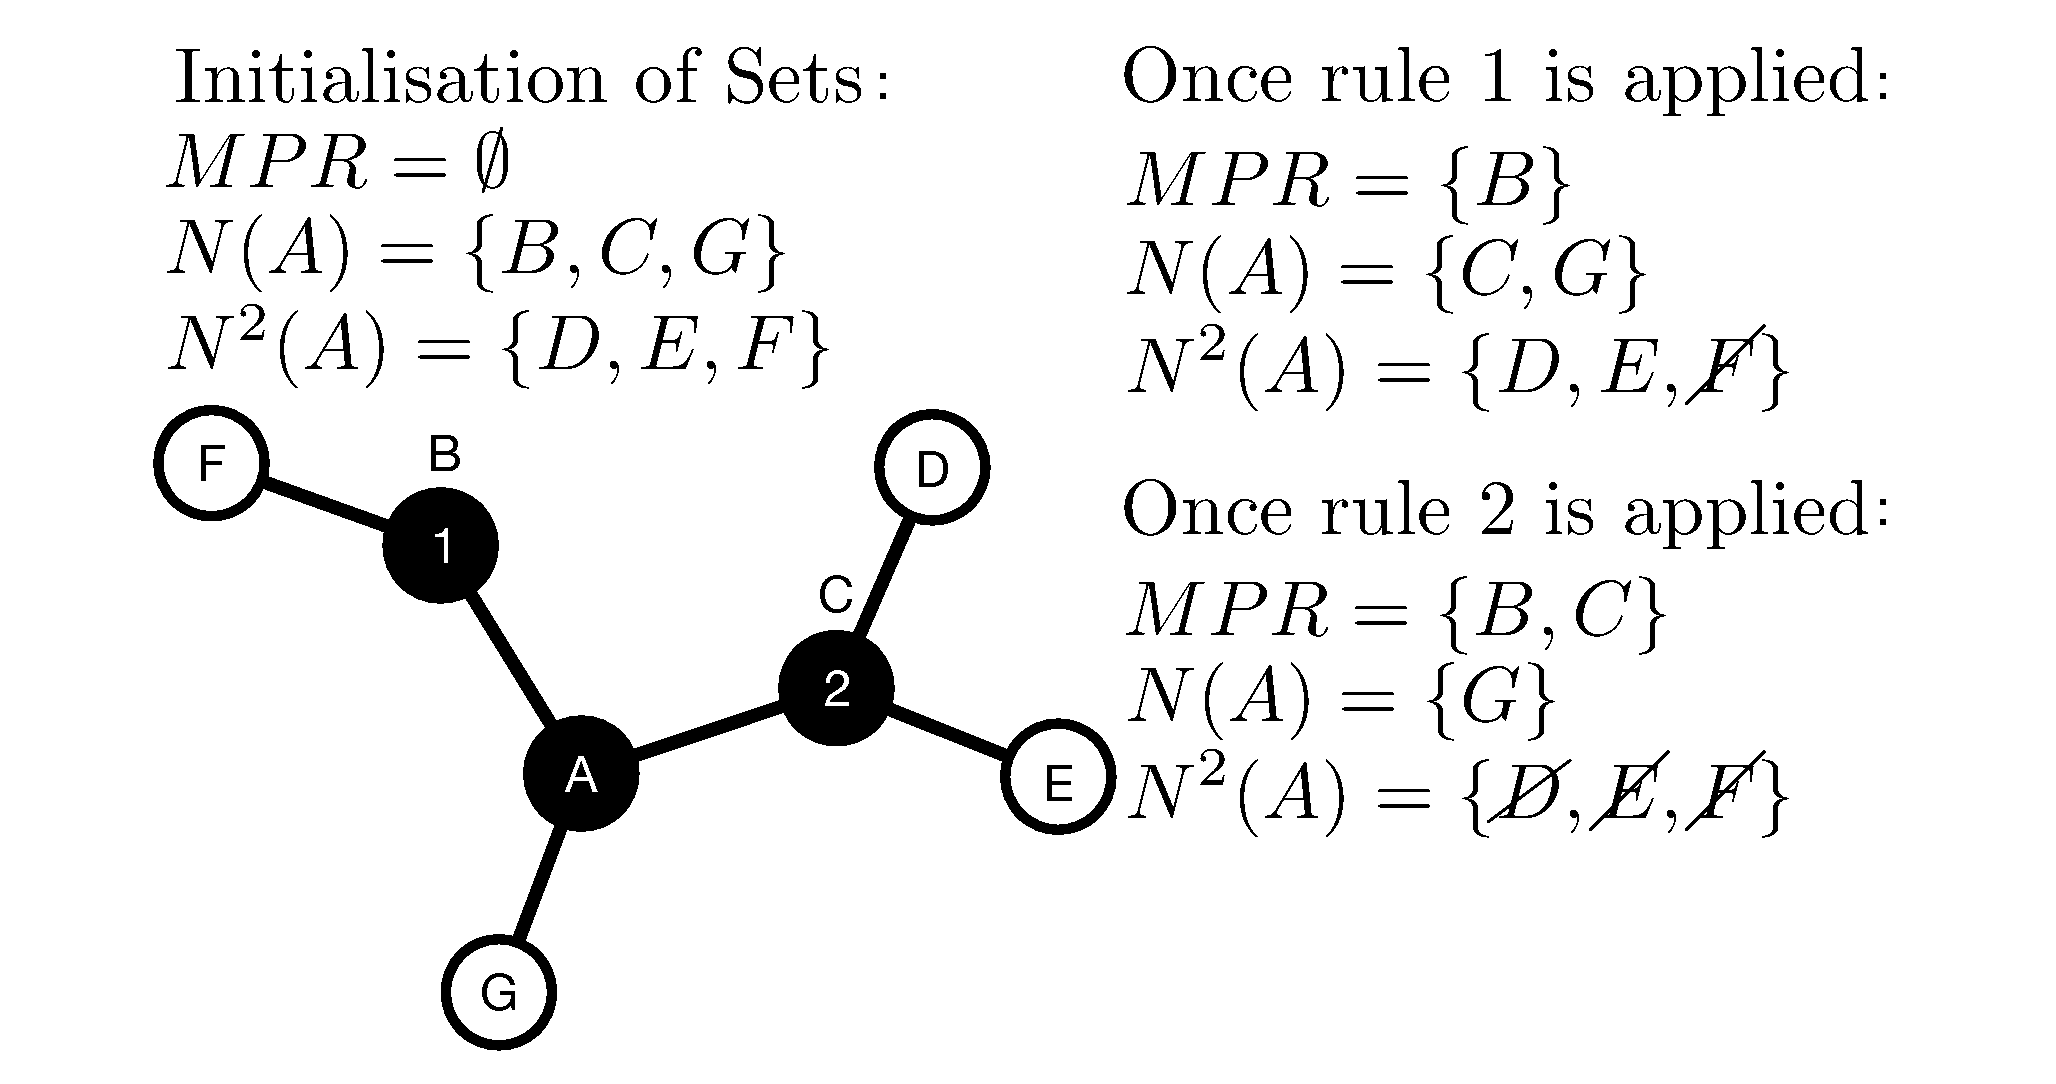
\includegraphics[width=\linewidth]{fig/explainingbackbone_b.pdf}	
	  \end{minipage}
	}
	~
	\subfigure[Backbone of 3 nodes shown by the black filled-in circles.] {
    \label{fig:explaining-backbone:b}
    \begin{minipage}[t]{\linewidth}
      \centering
	    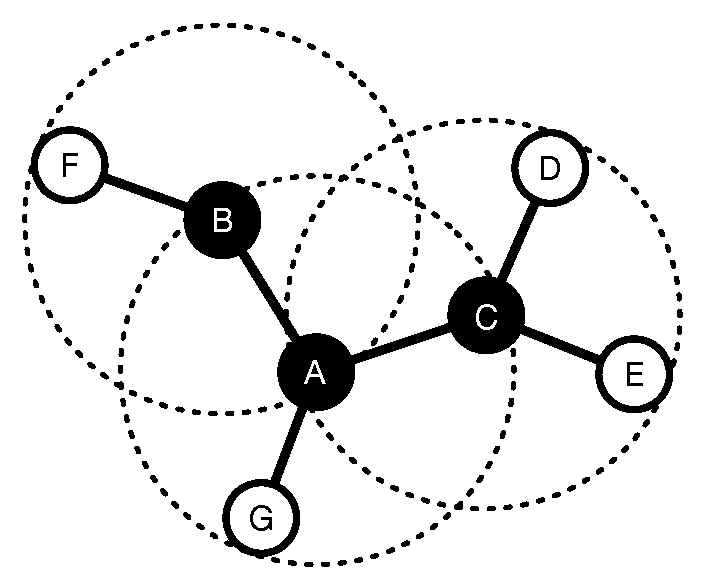
\includegraphics[scale=0.42]{fig/explainingbackbone_a.pdf}	
	  \end{minipage}
	}
	\caption{Virtual topology to reach 100\% reachability in one MANET.}
	\label{fig:explaining-backbone}
\end{figure}

\paragraph{MPR} The CDS obtained in~\cite{Qayyum2002} is called a MPR set.
%
Nodes start with an empty $MPR$ set having the knowledge of their one-hop and two-hop neighbors, represented by $N$ and $N^{2}$ respectively, thanks to previous exchanges of control messages.
%
The procedure to find relay nodes is two-fold.
%
Firstly, any one-hop neighbor $n \in N$ will belong to $MPR$ if $n$ is a unique neighbor of some other node at $N^{2}$.
%
Secondly, while the current MPR set do not cover all nodes at $N^{2}$, we iterate over each remaining neighbor $n \in N$ and we count how many two-hop neighbors are $n$ covers.
%
$n$ will be a relay node only if the number of covered two-hop neighbors is maximal.
%
Figure~\ref{fig:explaining-backbone:a} shows the steps taken by node $A$ to compute its $MPR$ set.
%
Once $A$ receives its one-hop and two-hop neighbors, node $B$ is marked as relay node because it is the unique neighbor of $F$ (first rule).
%
The second rule indicates that node $C$ must be part of the $MPR$ set, because the number of covered two-hop neighbors (i. e. two) is bigger than those neighbors cover by $G$ (which is zero).

\paragraph{CDS-based technique}
The decentralize algorithm in~\cite{Wu2001}, firstly approximates one CDS via a marking procedure and secondly, the number of relay nodes is minimized.
%
As in MPR, data about one-hop and two-hop neighbors is required. 
%
\changed{The marking procedure consist of identifying unconnected neighbors, if node $n$ realize that any pair of its neighbors is unconnected then, $n$ marks itself as forwarding node.}
\deleted{The marking procedure simply identifies whether one node $n$ has any pair of neighbors that are unconnected, $n$ marks itself as a relay node if this condition takes place.}
%
For instance, in Figure~\ref{fig:explaining-backbone:b} $A$ marks itself as relay node because nodes $B$ and $G$ are unconnected.
%
To reduce the elements of one CDS, obtained by the marking procedure, authors in~\cite{Wu2001} take into consideration either \textit{the degree of nodes} or \textit{the remaining energy in nodes' batteries}.
%
We chose the former approach to be fair in the comparison with MPR.

%
The node-degree-based rules are operations of first-order logic between the one-hop and two-hop sets of nodes' neighbors.
%
Due to the lack of space, we claim that our current implementation of the \textit{CDS-based technique} follows rules 2 and 2a (further details about these rules are found in~\cite{Wu2001}).


%As typically found with CDS-based approaches, during the flooding operation, nodes retransmit a message only if they have been marked as members of the CDS.
%As example of rules, we present the first two proposed in~\cite{Wu2001}.
%Notice that in the definition of such rules $\textit{nd}(v)$ is the node degree of $v$, $\textit{id}(v)$ is an unique identifier assigned to $v$ and $N\left[v\right] = N(v) \cup \lbrace v \rbrace$ where $N(v)$ is the set of neighbors of $v$:
%
%\begin{enumerate}
%	\item A node is marked if it has two unconnected neighbors. That is, $\exists u, w \in N(v), u \notin N(w)  \quad \textit{and} \quad w \notin N(w)$.
%	\item Consider two marked vertices $v$ and $u$. Then, $v$ is unmarked if one of the following conditions holds:
%	\begin{itemize}
%		\item $N\left[v\right] \subseteq N\left[u\right] \quad \textit{and} \quad \textit{nd}(v) < \textit{nd}(u)$.
%		\item $N\left[v\right] \subseteq N\left[u\right] \quad \textit{and} \quad \textit{nd}(v) = \textit{nd}(u) \quad \textit{and} \quad \\ \textit{id}(v) < \textit{id}(u)$.
%	\end{itemize}
%\end{enumerate} 

\subsection{Context-aware and context-oblivious algorithms}
Using a virtual topology implies an overload on the communication medium due to the constant exchange of control messages.
%
When nodes move, the frequency on sending these messages must be increased to keep a virtual topology with the correct set of relay nodes.
%
This results in a higher probability of collisions.
%
Moreover, our study considers a second category of broadcast protocols that do not require the exchange of control messages to build a virtual topology, instead, data is piggybacked in messages before their retransmission.
%
This data could be either context-oblivious or context-aware.
%
The former forwards messages with a predefine probability while the latter use knowledge about the current state of the network (for example, nodes' density).
%
%Particularly, when nodes move
%In some situations, creating and maintaining the underlying virtual topology is too costly or simply not feasible, in particular when the mobility of nodes would make a topology obsolete before it could be put to actual use.
%Thus, some protocols do not rely on any underlying topology. 
% Instead, they either use no information about the local node context, or only information that can be piggybacked with the dissemination messages.
%Some protocols use their local \textit{context} to decide if a node should retransmit a message.
%For instance, nodes can consider, among others, the number of neighbors, their mobility speed, how many neighbors have received a message~\cite{Ovalle-Martinez2006}, and the direction of the last sender of a received message.
%
%Since this contextual information varies over time, these algorithms often delay the retransmissions of a message until they can guarantee that doing so is strictly required.
%As the contextual data may depend on the variable time, a node may choose to retransmit a message at time $t_0$ and avoid doing so at $t_0+\delta t$.\laurent{not sure to get it}
%This approach usually saves energy and bandwidth, but it has a negative impact on other performance metrics as we discuss in Section~\ref{sec:evaluation}. 

%
\paragraph{Probabilistic Flooding} This is a context-aware and context-oblivious approach~\cite{Cartigny:2003:BNR:2727141.2727459} that uses information about one-hop neighbors and a probability to perform retransmissions.
%
Nodes retransmit messages based on the distance among neighbors and a probabilistic scheme.
%
This differs from the canonical probabilistic approach where every node in the network has the same probability of retransmitting a message regardless of the density.
%
The probability of retransmitting a message decreases as the local density increases.
%The rationale is that the neighbors of a node are likely closely packed in a dense area if the number of neighbors is large.

\paragraph{ABBA} Area-based beacon-less protocol~\cite{Ovalle-Martinez2006}.
The flooding process in ABBA is controlled in both space and time.
%
This algorithm requires nodes to know their physical location in addition to the transmission range of nodes' radio.
%
When one broadcast message $M$ is received, nodes compute the angle $\alpha$ covered by this reception.
%
Note that $\alpha$ is paired to a unique message.
%
$M$ is scheduled for being retransmitted after $T$ seconds, this timer is computed as follows $T = T_\textit{max} - T_\textit{max}\frac{\alpha}{2\pi}$, where $T_\textit{max}$ is a fixed upper bound that represents the maximum waiting time.
%
Prior of a new reception of $M$ before $T$ seconds, nodes cancel the current timer and schedule a new one.
%
In other words, the bigger the angle covered by message receptions, the shorter the time to wait before performing retransmissions.
%
With one exception, message retransmissions are canceled if $\alpha$ reaches a value of $2\pi$.


%Combining these two values, the authors propose a protocol that aims at delivering a full coverage with relatively low number of relay nodes. \er{i rephrased the previous but it reads as a judgment of the protocol, while we aim at being neutral}
%However, although the protocol requires both \textit{HELLO} messages and piggybacking, no experiment is presented to discuss important metrics such as energy consumption. 

%\laurent{Explain and refer the following protocols}
%\begin{enumerate}
%	\item Area Based -- \textbf{dist2mean}
		
%\end{enumerate}

%\subsubsection{Context-Oblivious}


%The probabilistic flooding is a mix of two approaches. There are two branches in the last level. They don't make the distinction in the survey, but it is clear when you read the paper.
%In opposition to the \textit{context-aware} family, there are also \textit{context-oblivious} algorithms that do not require prior information about the node locality to decide on the retransmission operation.
%
%These protocols are in general easy to implement and have no limiting requirements such as knowing the location of nodes nor exchanging extra messages with control information.
%
%However, it has been shown that for some algorithms such as the \textit{basic probabilistic} approach this simplicity comes at the expenses of a low coverage~\cite{Ni:1999:BSP:313451.313525}.
%
%In this paper, we are only considering one protocol in this class, the \textit{simple flooding}. 
%\er{this is a bit strange, again, to give opinions about the protocols while we intend to stay neutral.}



The diversity of algorithms to broadcast in MANETs is vast and choosing one approach to cope with a particular deployment scenario is a challenging task.
%
While some evaluations have been proposed to compare existing approaches, they usually target fixed scenarios; this avoids its use in other contexts.
%
In this work, our goal is to define an experimental framework to fairly assess representative algorithms  to broadcast in MANETs. 
%
In the next section, we discuss previous works one can find in the literature.
